\documentclass{article}
% option ``report'' puts title on separate page

\usepackage{amsmath}
\usepackage[pdftex]{graphicx}

\begin{document}

\title{WS5: Root Finding}
\author{Jackie Villadsen}
\date{\today}
\maketitle


\section{Eccentric Anomaly}
\begin{figure}[h]
  \begin{center}
     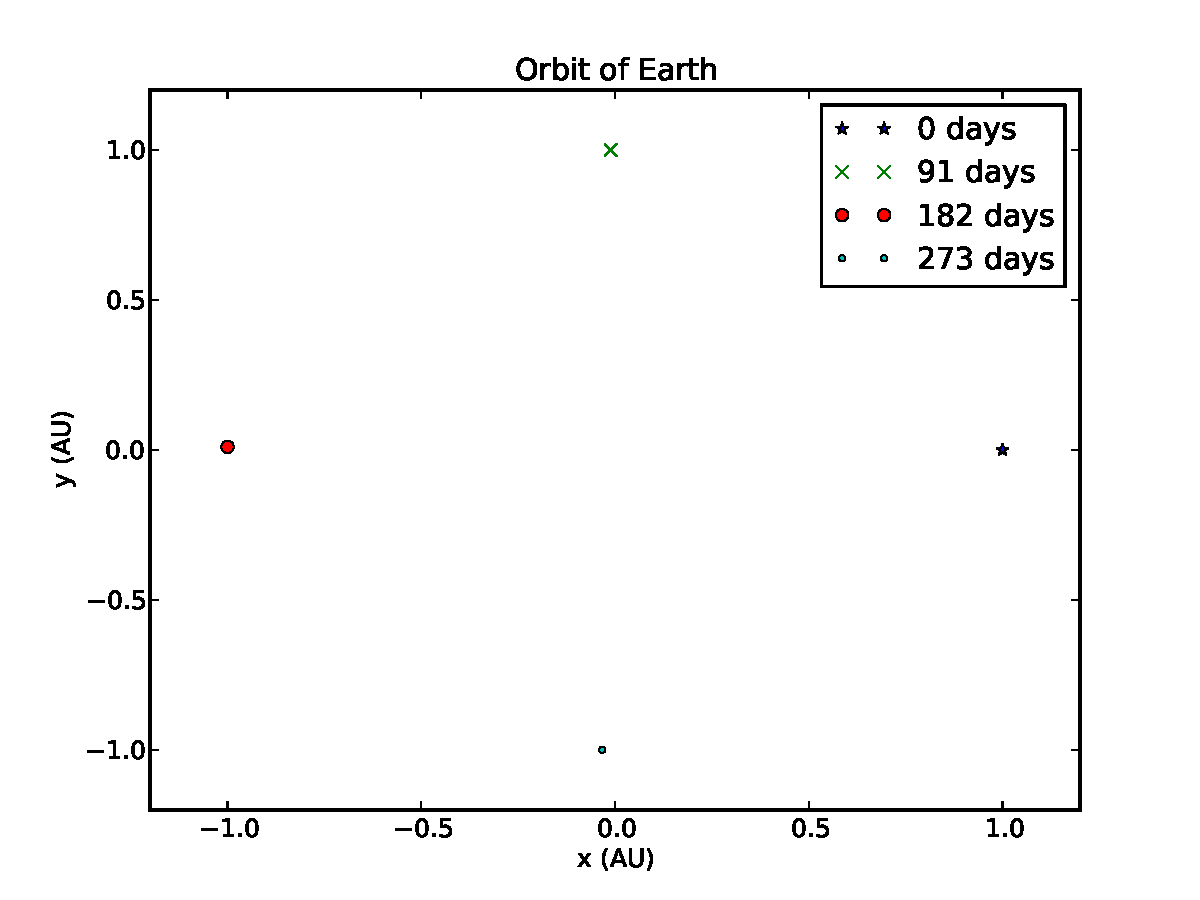
\includegraphics[width=\textwidth]{orbit0167}
  \end{center}
  \caption{The position of Earth in its orbit at 0, 91, 182, and 273 days, for its current eccentricity of 0.0167.}
  \label{fig:low_e}
\end{figure}

\begin{figure}[h]
  \begin{center}
     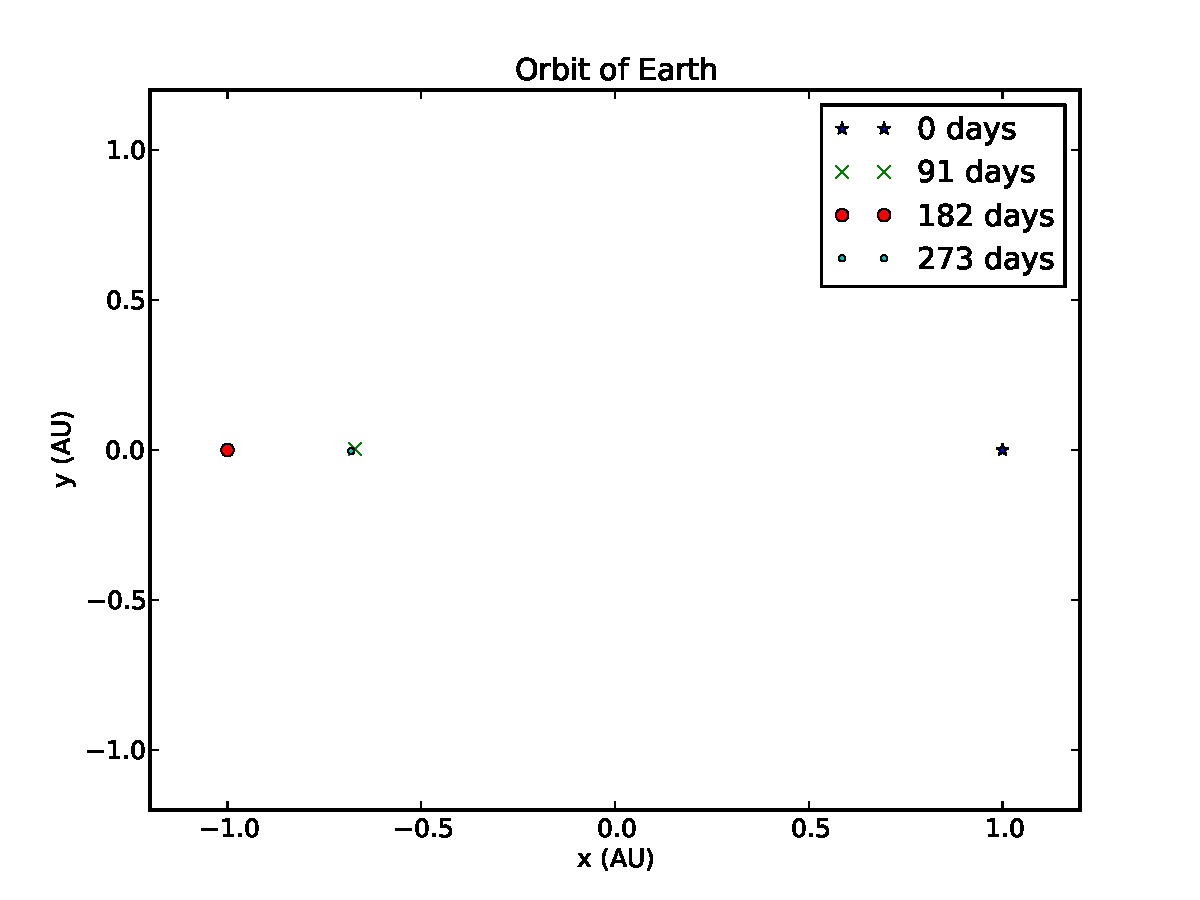
\includegraphics[width=\textwidth]{orbit99999}
  \end{center}
  \caption{The position of Earth in its orbit at 0, 91, 182, and 273 days, if its eccentricity were changed to 0.99999.}
  \label{fig:high_e}
\end{figure}

I used Newton's method to solve for the eccentric anomaly at different times in Earth's orbit.  Figure \ref{fig:low_e} shows
the positions of Earth at t=0 days (perihelion), 91 days, 182 days, and 273 days, for its current eccentricity of 0.0167.
Figure \ref{fig:high_e} shows the position of Earth at the same times if its eccentricity were changed to 0.99999.
Table \ref{tab:niter} shows the number of iterations needed to converge to a fractional error less than $10^{-10}$ for each
eccentricity, depending on the initial guess used for E.  For $E_0=0$, the number of iterations increased a lot with the
eccentricity.  However, for $E_0={\Omega}t$, the number of iterations remained quite low even for high eccentricity.

\begin{table}[p]
\centering
\begin{tabular}{|l|l|l|l|l|}
\hline
Time t (days) & $e=0.0167, E_0=0$ & $e=0.0167, E_0={\Omega}t$ & $e=0.99999, E_0=0$ & $e=0.99999, E_0={\Omega}t$ \\
\hline
0 & 1 & 1 & 1 & 1 \\
91 & 5 & 4 & 68 & 6 \\
182 & 4 & 3 & 35 & 3 \\
273 & 5 & 4 & 106 & 6 \\
\hline
\end{tabular}
\caption{This table shows the number of iterations needed to converge on the root E(t) using Newton's method, for low and high
eccentricity, and for using an initial guess of E=0 vs. a more intelligent initial guess of $E={\Omega}t$.}
\label{tab:niter}
\end{table}

\section{Polynomials with Multiple Roots}
I used the Durand-Kerner Method to solve for all the complex roots of any polynomial simultaneously.  The Durand-Kerner method
relies on the fact that the polynomial can be factored into the form:
\begin{equation}
	f(x) = \prod_i (x - r_i)
\end{equation}
where $r_i$ are the roots of the polynomial.

To obtain the n roots of a polynomial of degree n, I started with guesses: $r_i|_0 = (0.4 + 0.9j)^i$, as suggested by
Wikipedia.  These initial guesses are
arbitrary but fulfill the requirement that only one of them is a real number or a root of unity (i=0).

I then iterated forwards using the expression below, for 100 iterations (I found it difficult to set up a convergence
criterion for complex numbers, so instead I picked an arbitrary large number of iterations):
\begin{equation}
	r_i|_{n+1} = r_i|_n - \frac{f(r_i|_n)}{\prod_{i{\neq}j} (r_i|_n - r_j|_n)}
\end{equation}

For the polynomial given in the worksheet, $f(x)=3x^5+5x^4-x^3$, I obtained three roots whose real and imaginary components were
of order $10^{-18}$, corresponding to the three zero roots of the polynomial.  The other two roots were 0.1805 and -1.847 (with imaginary parts
of order $10^{-49}$ or less), which are the roots of the quadratic obtained by dividing by $x^3$.

I also tested my algorithm on a 3rd-degree polynomial given on Wikipedia, $f(x)=x^3-3x^2+3x-5$, successfully recovering the one real root, 2.5874,
and the two imaginary roots, 0.206$\pm$1.375j.  Finally, I tested my algorithm on the simple example $f(x)=x^2$, which yielded two roots whose
complex and imaginary parts were both of order $10^{-30}$ (essentially zero).

\end{document}